\documentclass[1p]{elsarticle_modified}
%\bibliographystyle{elsarticle-num}

%\usepackage[colorlinks]{hyperref}
%\usepackage{abbrmath_seonhwa} %\Abb, \Ascr, \Acal ,\Abf, \Afrak
\usepackage{amsfonts}
\usepackage{amssymb}
\usepackage{amsmath}
\usepackage{amsthm}
\usepackage{scalefnt}
\usepackage{amsbsy}
\usepackage{kotex}
\usepackage{caption}
\usepackage{subfig}
\usepackage{color}
\usepackage{graphicx}
\usepackage{xcolor} %% white, black, red, green, blue, cyan, magenta, yellow
\usepackage{float}
\usepackage{setspace}
\usepackage{hyperref}

\usepackage{tikz}
\usetikzlibrary{arrows}

\usepackage{multirow}
\usepackage{array} % fixed length table
\usepackage{hhline}

%%%%%%%%%%%%%%%%%%%%%
\makeatletter
\renewcommand*\env@matrix[1][\arraystretch]{%
	\edef\arraystretch{#1}%
	\hskip -\arraycolsep
	\let\@ifnextchar\new@ifnextchar
	\array{*\c@MaxMatrixCols c}}
\makeatother %https://tex.stackexchange.com/questions/14071/how-can-i-increase-the-line-spacing-in-a-matrix
%%%%%%%%%%%%%%%

\usepackage[normalem]{ulem}

\newcommand{\msout}[1]{\ifmmode\text{\sout{\ensuremath{#1}}}\else\sout{#1}\fi}
%SOURCE: \msout is \stkout macro in https://tex.stackexchange.com/questions/20609/strikeout-in-math-mode

\newcommand{\cancel}[1]{
	\ifmmode
	{\color{red}\msout{#1}}
	\else
	{\color{red}\sout{#1}}
	\fi
}

\newcommand{\add}[1]{
	{\color{blue}\uwave{#1}}
}

\newcommand{\replace}[2]{
	\ifmmode
	{\color{red}\msout{#1}}{\color{blue}\uwave{#2}}
	\else
	{\color{red}\sout{#1}}{\color{blue}\uwave{#2}}
	\fi
}

\newcommand{\Sol}{\mathcal{S}} %segment
\newcommand{\D}{D} %diagram
\newcommand{\A}{\mathcal{A}} %arc


%%%%%%%%%%%%%%%%%%%%%%%%%%%%%5 test

\def\sl{\operatorname{\textup{SL}}(2,\Cbb)}
\def\psl{\operatorname{\textup{PSL}}(2,\Cbb)}
\def\quan{\mkern 1mu \triangleright \mkern 1mu}

\theoremstyle{definition}
\newtheorem{thm}{Theorem}[section]
\newtheorem{prop}[thm]{Proposition}
\newtheorem{lem}[thm]{Lemma}
\newtheorem{ques}[thm]{Question}
\newtheorem{cor}[thm]{Corollary}
\newtheorem{defn}[thm]{Definition}
\newtheorem{exam}[thm]{Example}
\newtheorem{rmk}[thm]{Remark}
\newtheorem{alg}[thm]{Algorithm}

\newcommand{\I}{\sqrt{-1}}
\begin{document}

%\begin{frontmatter}
%
%\title{Boundary parabolic representations of knots up to 8 crossings}
%
%%% Group authors per affiliation:
%\author{Yunhi Cho} 
%\address{Department of Mathematics, University of Seoul, Seoul, Korea}
%\ead{yhcho@uos.ac.kr}
%
%
%\author{Seonhwa Kim} %\fnref{s_kim}}
%\address{Center for Geometry and Physics, Institute for Basic Science, Pohang, 37673, Korea}
%\ead{ryeona17@ibs.re.kr}
%
%\author{Hyuk Kim}
%\address{Department of Mathematical Sciences, Seoul National University, Seoul 08826, Korea}
%\ead{hyukkim@snu.ac.kr}
%
%\author{Seokbeom Yoon}
%\address{Department of Mathematical Sciences, Seoul National University, Seoul, 08826,  Korea}
%\ead{sbyoon15@snu.ac.kr}
%
%\begin{abstract}
%We find all boundary parabolic representation of knots up to 8 crossings.
%
%\end{abstract}
%\begin{keyword}
%    \MSC[2010] 57M25 
%\end{keyword}
%
%\end{frontmatter}

%\linenumbers
%\tableofcontents
%
\newcommand\colored[1]{\textcolor{white}{\rule[-0.35ex]{0.8em}{1.4ex}}\kern-0.8em\color{red} #1}%
%\newcommand\colored[1]{\textcolor{white}{ #1}\kern-2.17ex	\textcolor{white}{ #1}\kern-1.81ex	\textcolor{white}{ #1}\kern-2.15ex\color{red}#1	}

{\Large $\underline{11n_{14}~(K11n_{14})}$}

\setlength{\tabcolsep}{10pt}
\renewcommand{\arraystretch}{1.6}
\vspace{1cm}\begin{tabular}{m{100pt}>{\centering\arraybackslash}m{274pt}}
\multirow{5}{120pt}{
	\centering
	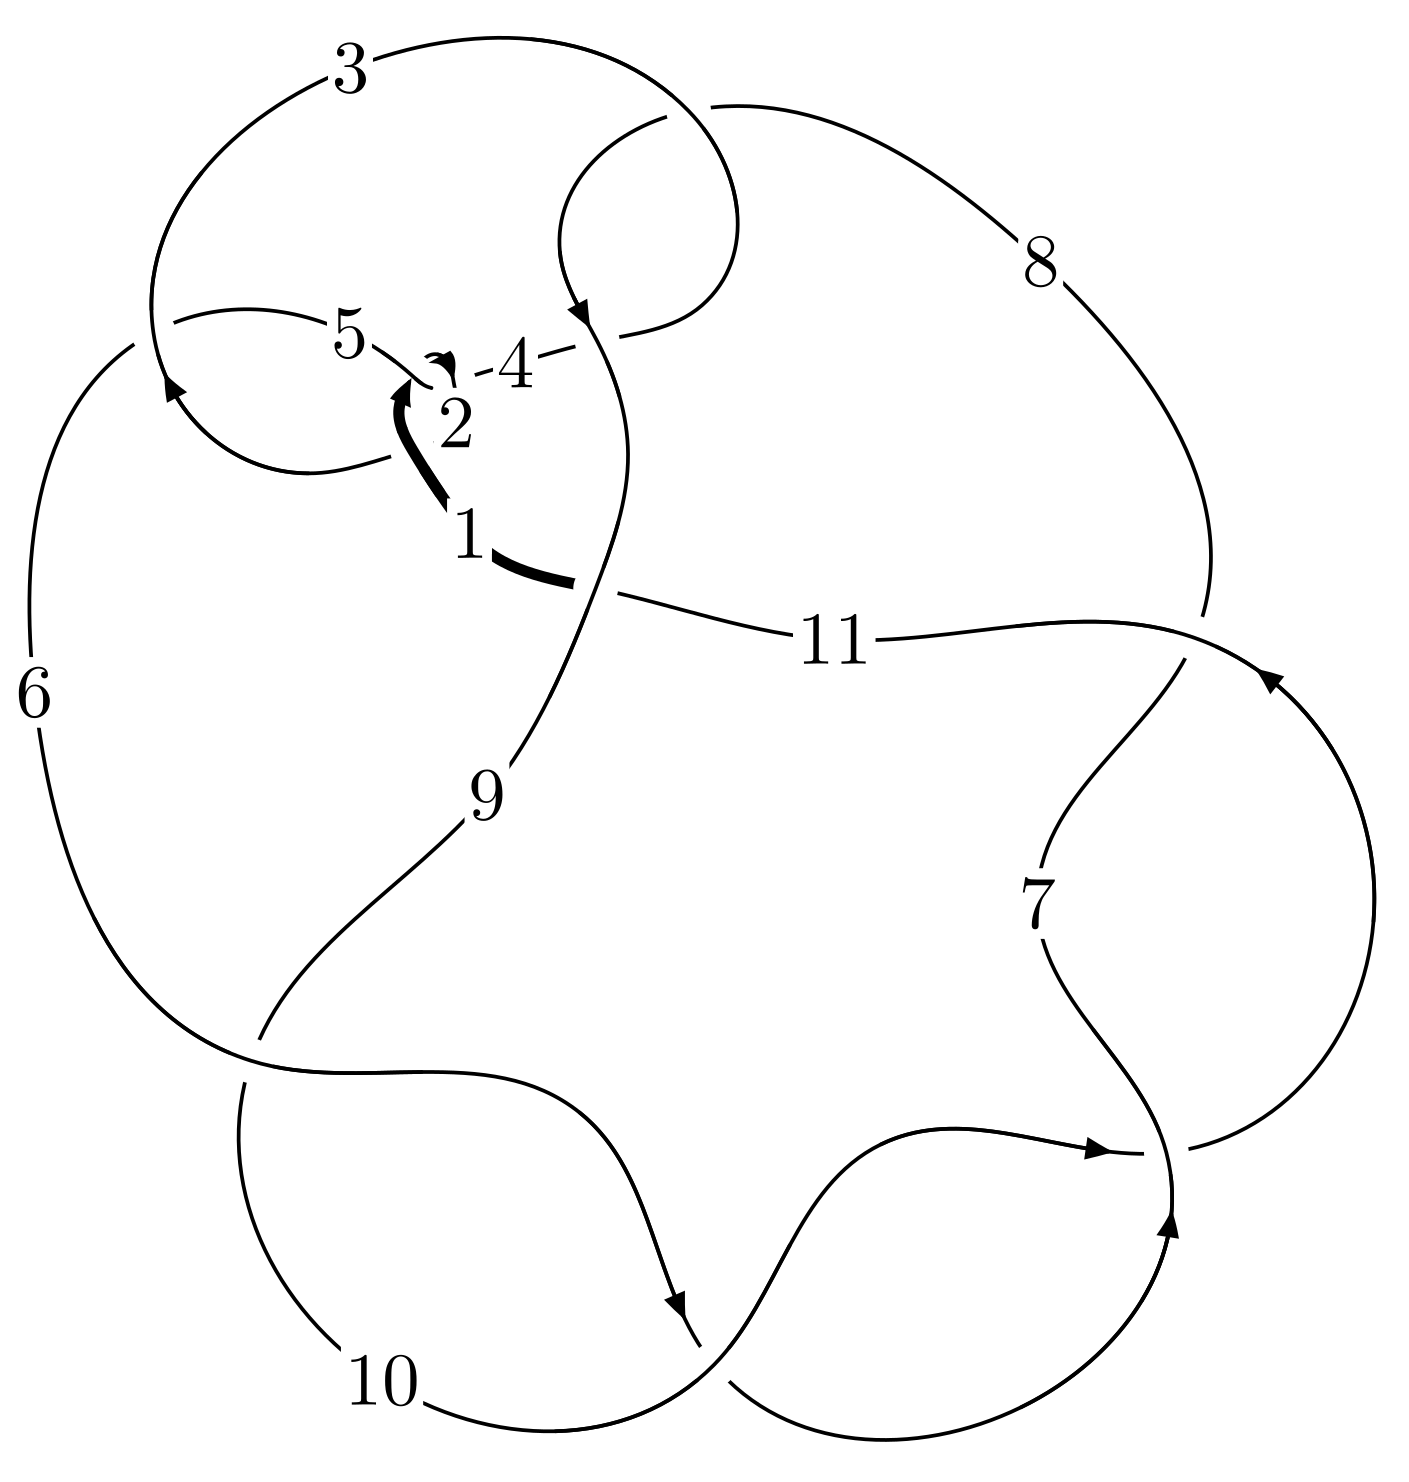
\includegraphics[width=112pt]{../../../GIT/diagram.site/Diagrams/png/630_11n_14.png}\\
\ \ \ A knot diagram\footnotemark}&
\allowdisplaybreaks
\textbf{Linearized knot diagam} \\
\cline{2-2}
 &
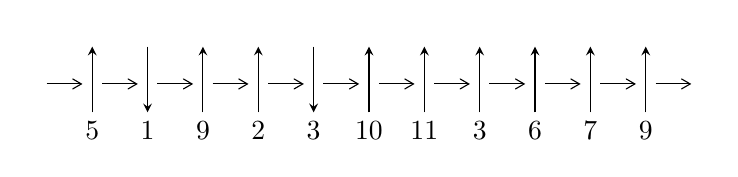
\begin{tikzpicture}[x=20pt, y=17pt]
	% nodes
	\node (C0) at (0, 0) {};
	\node (C1) at (1, 0) {};
	\node (C1U) at (1, +1) {};
	\node (C1D) at (1, -1) {5};

	\node (C2) at (2, 0) {};
	\node (C2U) at (2, +1) {};
	\node (C2D) at (2, -1) {1};

	\node (C3) at (3, 0) {};
	\node (C3U) at (3, +1) {};
	\node (C3D) at (3, -1) {9};

	\node (C4) at (4, 0) {};
	\node (C4U) at (4, +1) {};
	\node (C4D) at (4, -1) {2};

	\node (C5) at (5, 0) {};
	\node (C5U) at (5, +1) {};
	\node (C5D) at (5, -1) {3};

	\node (C6) at (6, 0) {};
	\node (C6U) at (6, +1) {};
	\node (C6D) at (6, -1) {10};

	\node (C7) at (7, 0) {};
	\node (C7U) at (7, +1) {};
	\node (C7D) at (7, -1) {11};

	\node (C8) at (8, 0) {};
	\node (C8U) at (8, +1) {};
	\node (C8D) at (8, -1) {3};

	\node (C9) at (9, 0) {};
	\node (C9U) at (9, +1) {};
	\node (C9D) at (9, -1) {6};

	\node (C10) at (10, 0) {};
	\node (C10U) at (10, +1) {};
	\node (C10D) at (10, -1) {7};

	\node (C11) at (11, 0) {};
	\node (C11U) at (11, +1) {};
	\node (C11D) at (11, -1) {9};
	\node (C12) at (12, 0) {};

	% arrows
	\draw[->,>={angle 60}]
	(C0) edge (C1) (C1) edge (C2) (C2) edge (C3) (C3) edge (C4) (C4) edge (C5) (C5) edge (C6) (C6) edge (C7) (C7) edge (C8) (C8) edge (C9) (C9) edge (C10) (C10) edge (C11) (C11) edge (C12) ;	\draw[->,>=stealth]
	(C1D) edge (C1U) (C2U) edge (C2D) (C3D) edge (C3U) (C4D) edge (C4U) (C5U) edge (C5D) (C6D) edge (C6U) (C7D) edge (C7U) (C8D) edge (C8U) (C9D) edge (C9U) (C10D) edge (C10U) (C11D) edge (C11U) ;
	\end{tikzpicture} \\
\hhline{~~} \\& 
\textbf{Solving Sequence} \\ \cline{2-2} 
 &
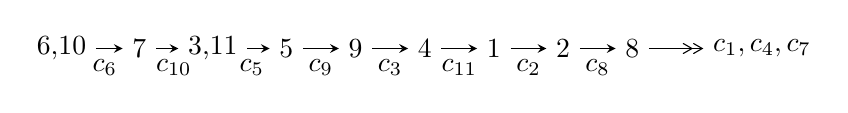
\begin{tikzpicture}[x=25pt, y=7pt]
	% node
	\node (A0) at (-1/8, 0) {6,10};
	\node (A1) at (1, 0) {7};
	\node (A2) at (33/16, 0) {3,11};
	\node (A3) at (25/8, 0) {5};
	\node (A4) at (33/8, 0) {9};
	\node (A5) at (41/8, 0) {4};
	\node (A6) at (49/8, 0) {1};
	\node (A7) at (57/8, 0) {2};
	\node (A8) at (65/8, 0) {8};
	\node (C1) at (1/2, -1) {$c_{6}$};
	\node (C2) at (3/2, -1) {$c_{10}$};
	\node (C3) at (21/8, -1) {$c_{5}$};
	\node (C4) at (29/8, -1) {$c_{9}$};
	\node (C5) at (37/8, -1) {$c_{3}$};
	\node (C6) at (45/8, -1) {$c_{11}$};
	\node (C7) at (53/8, -1) {$c_{2}$};
	\node (C8) at (61/8, -1) {$c_{8}$};
	\node (A9) at (10, 0) {$c_{1},c_{4},c_{7}$};

	% edge
	\draw[->,>=stealth]	
	(A0) edge (A1) (A1) edge (A2) (A2) edge (A3) (A3) edge (A4) (A4) edge (A5) (A5) edge (A6) (A6) edge (A7) (A7) edge (A8) ;
	\draw[->>,>={angle 60}]	
	(A8) edge (A9);
\end{tikzpicture} \\ 

\end{tabular} \\

\footnotetext{
The image of knot diagram is generated by the software ``\textbf{Draw programme}" developed by Andrew Bartholomew(\url{http://www.layer8.co.uk/maths/draw/index.htm\#Running-draw}), where we modified some parts for our purpose(\url{https://github.com/CATsTAILs/LinksPainter}).
}\phantom \\ \newline 
\centering \textbf{Ideals for irreducible components\footnotemark of $X_{\text{par}}$} 
 
\begin{align*}
I^u_{1}&=\langle 
-3 u^{25}-6 u^{24}+\cdots+2 b-7 u,\;7 u^{25}+14 u^{24}+\cdots+2 a+9 u,\;u^{26}+3 u^{25}+\cdots+u-1\rangle \\
I^u_{2}&=\langle 
b+a,\;a^2- a+1,\;u^2- u-1\rangle \\
\\
\end{align*}
\raggedright * 2 irreducible components of $\dim_{\mathbb{C}}=0$, with total 30 representations.\\
\footnotetext{All coefficients of polynomials are rational numbers. But the coefficients are sometimes approximated in decimal forms when there is not enough margin.}
\newpage
\renewcommand{\arraystretch}{1}
\centering \section*{I. $I^u_{1}= \langle -3 u^{25}-6 u^{24}+\cdots+2 b-7 u,\;7 u^{25}+14 u^{24}+\cdots+2 a+9 u,\;u^{26}+3 u^{25}+\cdots+u-1 \rangle$}
\flushleft \textbf{(i) Arc colorings}\\
\begin{tabular}{m{7pt} m{180pt} m{7pt} m{180pt} }
\flushright $a_{6}=$&$\begin{pmatrix}1\\0\end{pmatrix}$ \\
\flushright $a_{10}=$&$\begin{pmatrix}0\\u\end{pmatrix}$ \\
\flushright $a_{7}=$&$\begin{pmatrix}1\\- u^2\end{pmatrix}$ \\
\flushright $a_{3}=$&$\begin{pmatrix}-\frac{7}{2} u^{25}-7 u^{24}+\cdots-2 u^2-\frac{9}{2} u\\\frac{3}{2} u^{25}+3 u^{24}+\cdots+u^2+\frac{7}{2} u\end{pmatrix}$ \\
\flushright $a_{11}=$&$\begin{pmatrix}u\\- u^3+u\end{pmatrix}$ \\
\flushright $a_{5}=$&$\begin{pmatrix}\frac{1}{2} u^{25}+u^{24}+\cdots-4 u^2-\frac{5}{2} u\\-\frac{1}{2} u^{25}- u^{24}+\cdots+4 u^2+\frac{1}{2} u\end{pmatrix}$ \\
\flushright $a_{9}=$&$\begin{pmatrix}- u\\u\end{pmatrix}$ \\
\flushright $a_{4}=$&$\begin{pmatrix}-\frac{13}{2} u^{25}-12 u^{24}+\cdots-\frac{17}{2} u+2\\\frac{9}{2} u^{25}+8 u^{24}+\cdots+\frac{15}{2} u-2\end{pmatrix}$ \\
\flushright $a_{1}=$&$\begin{pmatrix}- u^5+2 u^3+u\\u^5-3 u^3+u\end{pmatrix}$ \\
\flushright $a_{2}=$&$\begin{pmatrix}-6 u^{25}-10 u^{24}+\cdots-6 u+2\\\frac{11}{2} u^{25}+9 u^{24}+\cdots+\frac{15}{2} u-2\end{pmatrix}$ \\
\flushright $a_{8}=$&$\begin{pmatrix}- u^2+1\\u^4-2 u^2\end{pmatrix}$\\ \flushright $a_{8}=$&$\begin{pmatrix}- u^2+1\\u^4-2 u^2\end{pmatrix}$\\&\end{tabular}
\flushleft \textbf{(ii) Obstruction class $= -1$}\\~\\
\flushleft \textbf{(iii) Cusp Shapes $= \frac{5}{2} u^{25}+4 u^{24}-\frac{57}{2} u^{23}-41 u^{22}+\frac{277}{2} u^{21}+\frac{305}{2} u^{20}-391 u^{19}-205 u^{18}+\frac{1475}{2} u^{17}-141 u^{16}-910 u^{15}+742 u^{14}+464 u^{13}-\frac{1721}{2} u^{12}+374 u^{11}+381 u^{10}-512 u^9+147 u^8+\frac{229}{2} u^7-247 u^6-\frac{49}{2} u^5+\frac{29}{2} u^4-53 u^3-27 u^2-\frac{29}{2} u+9$}\\~\\
\newpage\renewcommand{\arraystretch}{1}
\flushleft \textbf{(iv) u-Polynomials at the component}\newline \\
\begin{tabular}{m{50pt}|m{274pt}}
Crossings & \hspace{64pt}u-Polynomials at each crossing \\
\hline $$\begin{aligned}c_{1},c_{4}\end{aligned}$$&$\begin{aligned}
&u^{26}+3 u^{25}+\cdots-3 u+1
\end{aligned}$\\
\hline $$\begin{aligned}c_{2}\end{aligned}$$&$\begin{aligned}
&u^{26}+15 u^{25}+\cdots-23 u+1
\end{aligned}$\\
\hline $$\begin{aligned}c_{3},c_{8}\end{aligned}$$&$\begin{aligned}
&u^{26}- u^{25}+\cdots+16 u-16
\end{aligned}$\\
\hline $$\begin{aligned}c_{5}\end{aligned}$$&$\begin{aligned}
&u^{26}-3 u^{25}+\cdots-11 u+2
\end{aligned}$\\
\hline $$\begin{aligned}c_{6},c_{7},c_{9}\\c_{10}\end{aligned}$$&$\begin{aligned}
&u^{26}-3 u^{25}+\cdots- u-1
\end{aligned}$\\
\hline $$\begin{aligned}c_{11}\end{aligned}$$&$\begin{aligned}
&u^{26}+3 u^{25}+\cdots+3 u-1
\end{aligned}$\\
\hline
\end{tabular}\\~\\
\newpage\renewcommand{\arraystretch}{1}
\flushleft \textbf{(v) Riley Polynomials at the component}\newline \\
\begin{tabular}{m{50pt}|m{274pt}}
Crossings & \hspace{64pt}Riley Polynomials at each crossing \\
\hline $$\begin{aligned}c_{1},c_{4}\end{aligned}$$&$\begin{aligned}
&y^{26}+15 y^{25}+\cdots-23 y+1
\end{aligned}$\\
\hline $$\begin{aligned}c_{2}\end{aligned}$$&$\begin{aligned}
&y^{26}-5 y^{25}+\cdots-795 y+1
\end{aligned}$\\
\hline $$\begin{aligned}c_{3},c_{8}\end{aligned}$$&$\begin{aligned}
&y^{26}+25 y^{25}+\cdots+1664 y+256
\end{aligned}$\\
\hline $$\begin{aligned}c_{5}\end{aligned}$$&$\begin{aligned}
&y^{26}-25 y^{25}+\cdots+7 y+4
\end{aligned}$\\
\hline $$\begin{aligned}c_{6},c_{7},c_{9}\\c_{10}\end{aligned}$$&$\begin{aligned}
&y^{26}-29 y^{25}+\cdots-19 y+1
\end{aligned}$\\
\hline $$\begin{aligned}c_{11}\end{aligned}$$&$\begin{aligned}
&y^{26}+31 y^{25}+\cdots-19 y+1
\end{aligned}$\\
\hline
\end{tabular}\\~\\
\newpage\flushleft \textbf{(vi) Complex Volumes and Cusp Shapes}
$$\begin{array}{c|c|c}  
\text{Solutions to }I^u_{1}& \I (\text{vol} + \sqrt{-1}CS) & \text{Cusp shape}\\
 \hline 
\begin{aligned}
u &= \phantom{-}0.608473 + 0.715807 I \\
a &= \phantom{-}0.153590 - 1.045830 I \\
b &= -1.73126 + 0.24397 I\end{aligned}
 & -7.73283 + 7.28919 I & \phantom{-}4.65018 - 5.96812 I \\ \hline\begin{aligned}
u &= \phantom{-}0.608473 - 0.715807 I \\
a &= \phantom{-}0.153590 + 1.045830 I \\
b &= -1.73126 - 0.24397 I\end{aligned}
 & -7.73283 - 7.28919 I & \phantom{-}4.65018 + 5.96812 I \\ \hline\begin{aligned}
u &= \phantom{-}0.433445 + 0.761836 I \\
a &= -0.011324 - 1.102790 I \\
b &= -1.56800 + 0.06124 I\end{aligned}
 & -8.25588 - 2.37235 I & \phantom{-}3.41364 + 0.56644 I \\ \hline\begin{aligned}
u &= \phantom{-}0.433445 - 0.761836 I \\
a &= -0.011324 + 1.102790 I \\
b &= -1.56800 - 0.06124 I\end{aligned}
 & -8.25588 + 2.37235 I & \phantom{-}3.41364 - 0.56644 I \\ \hline\begin{aligned}
u &= \phantom{-}0.514434 + 0.670493 I \\
a &= -0.106433 + 1.146570 I \\
b &= \phantom{-}1.59480 - 0.23303 I\end{aligned}
 & -4.15442 + 2.25820 I & \phantom{-}7.09524 - 3.00458 I \\ \hline\begin{aligned}
u &= \phantom{-}0.514434 - 0.670493 I \\
a &= -0.106433 - 1.146570 I \\
b &= \phantom{-}1.59480 + 0.23303 I\end{aligned}
 & -4.15442 - 2.25820 I & \phantom{-}7.09524 + 3.00458 I \\ \hline\begin{aligned}
u &= -0.730522 + 0.264601 I \\
a &= -0.408112 - 0.721539 I \\
b &= -0.020892 - 0.242346 I\end{aligned}
 & \phantom{-}0.141642 - 0.491245 I & \phantom{-}7.19488 + 1.21216 I \\ \hline\begin{aligned}
u &= -0.730522 - 0.264601 I \\
a &= -0.408112 + 0.721539 I \\
b &= -0.020892 + 0.242346 I\end{aligned}
 & \phantom{-}0.141642 + 0.491245 I & \phantom{-}7.19488 - 1.21216 I \\ \hline\begin{aligned}
u &= \phantom{-}1.42824 + 0.09847 I \\
a &= -0.332202 + 0.112416 I \\
b &= \phantom{-}1.191590 - 0.262632 I\end{aligned}
 & \phantom{-}3.94867 + 3.99401 I & \phantom{-}9.09163 - 3.57778 I \\ \hline\begin{aligned}
u &= \phantom{-}1.42824 - 0.09847 I \\
a &= -0.332202 - 0.112416 I \\
b &= \phantom{-}1.191590 + 0.262632 I\end{aligned}
 & \phantom{-}3.94867 - 3.99401 I & \phantom{-}9.09163 + 3.57778 I\\
 \hline 
 \end{array}$$\newpage$$\begin{array}{c|c|c}  
\text{Solutions to }I^u_{1}& \I (\text{vol} + \sqrt{-1}CS) & \text{Cusp shape}\\
 \hline 
\begin{aligned}
u &= -1.47226 + 0.03460 I \\
a &= -0.29209 - 2.37542 I \\
b &= \phantom{-}0.36258 + 1.62911 I\end{aligned}
 & \phantom{-}6.47513 - 2.78553 I & \phantom{-}10.00226 + 3.18308 I \\ \hline\begin{aligned}
u &= -1.47226 - 0.03460 I \\
a &= -0.29209 + 2.37542 I \\
b &= \phantom{-}0.36258 - 1.62911 I\end{aligned}
 & \phantom{-}6.47513 + 2.78553 I & \phantom{-}10.00226 - 3.18308 I \\ \hline\begin{aligned}
u &= -1.45262 + 0.27035 I \\
a &= \phantom{-}0.87552 + 1.41378 I \\
b &= -1.239850 - 0.375242 I\end{aligned}
 & -2.20853 - 1.36342 I & \phantom{-}6.29553 + 0.38377 I \\ \hline\begin{aligned}
u &= -1.45262 - 0.27035 I \\
a &= \phantom{-}0.87552 - 1.41378 I \\
b &= -1.239850 + 0.375242 I\end{aligned}
 & -2.20853 + 1.36342 I & \phantom{-}6.29553 - 0.38377 I \\ \hline\begin{aligned}
u &= -0.230011 + 0.458848 I \\
a &= \phantom{-}0.727275 + 1.025970 I \\
b &= \phantom{-}0.536127 + 0.217517 I\end{aligned}
 & -1.40190 - 2.19157 I & \phantom{-}3.35211 + 5.42014 I \\ \hline\begin{aligned}
u &= -0.230011 - 0.458848 I \\
a &= \phantom{-}0.727275 - 1.025970 I \\
b &= \phantom{-}0.536127 - 0.217517 I\end{aligned}
 & -1.40190 + 2.19157 I & \phantom{-}3.35211 - 5.42014 I \\ \hline\begin{aligned}
u &= \phantom{-}1.49087\phantom{ +0.000000I} \\
a &= \phantom{-}0.257464\phantom{ +0.000000I} \\
b &= -0.956110\phantom{ +0.000000I}\end{aligned}
 & \phantom{-}7.14521\phantom{ +0.000000I} & \phantom{-}13.5410\phantom{ +0.000000I} \\ \hline\begin{aligned}
u &= -1.52539 + 0.21566 I \\
a &= -1.11758 - 1.58851 I \\
b &= \phantom{-}1.54625 + 0.70491 I\end{aligned}
 & \phantom{-}2.54423 - 5.47373 I & \phantom{-}10.67253 + 2.88121 I \\ \hline\begin{aligned}
u &= -1.52539 - 0.21566 I \\
a &= -1.11758 + 1.58851 I \\
b &= \phantom{-}1.54625 - 0.70491 I\end{aligned}
 & \phantom{-}2.54423 + 5.47373 I & \phantom{-}10.67253 - 2.88121 I \\ \hline\begin{aligned}
u &= -0.448296\phantom{ +0.000000I} \\
a &= -0.791985\phantom{ +0.000000I} \\
b &= -0.195879\phantom{ +0.000000I}\end{aligned}
 & \phantom{-}0.706372\phantom{ +0.000000I} & \phantom{-}14.0850\phantom{ +0.000000I}\\
 \hline 
 \end{array}$$\newpage$$\begin{array}{c|c|c}  
\text{Solutions to }I^u_{1}& \I (\text{vol} + \sqrt{-1}CS) & \text{Cusp shape}\\
 \hline 
\begin{aligned}
u &= -1.56905 + 0.24097 I \\
a &= \phantom{-}1.25395 + 1.44166 I \\
b &= -1.78957 - 0.55743 I\end{aligned}
 & -0.54439 - 10.83970 I & \phantom{-}8.04696 + 6.04188 I \\ \hline\begin{aligned}
u &= -1.56905 - 0.24097 I \\
a &= \phantom{-}1.25395 - 1.44166 I \\
b &= -1.78957 + 0.55743 I\end{aligned}
 & -0.54439 + 10.83970 I & \phantom{-}8.04696 - 6.04188 I \\ \hline\begin{aligned}
u &= \phantom{-}1.63847 + 0.03227 I \\
a &= \phantom{-}0.0580399 - 0.1115770 I \\
b &= -0.266246 + 0.474227 I\end{aligned}
 & \phantom{-}8.45818 + 1.37920 I & \phantom{-}7.00000 + 2.69707 I \\ \hline\begin{aligned}
u &= \phantom{-}1.63847 - 0.03227 I \\
a &= \phantom{-}0.0580399 + 0.1115770 I \\
b &= -0.266246 - 0.474227 I\end{aligned}
 & \phantom{-}8.45818 - 1.37920 I & \phantom{-}7.00000 - 2.69707 I \\ \hline\begin{aligned}
u &= \phantom{-}0.335499 + 0.109869 I \\
a &= -0.03337 + 2.42886 I \\
b &= \phantom{-}0.460465 - 1.052830 I\end{aligned}
 & \phantom{-}0.44924 + 2.24817 I & \phantom{-}0.24032 - 5.78182 I \\ \hline\begin{aligned}
u &= \phantom{-}0.335499 - 0.109869 I \\
a &= -0.03337 - 2.42886 I \\
b &= \phantom{-}0.460465 + 1.052830 I\end{aligned}
 & \phantom{-}0.44924 - 2.24817 I & \phantom{-}0.24032 + 5.78182 I\\
 \hline 
 \end{array}$$\newpage\newpage\renewcommand{\arraystretch}{1}
\centering \section*{II. $I^u_{2}= \langle b+a,\;a^2- a+1,\;u^2- u-1 \rangle$}
\flushleft \textbf{(i) Arc colorings}\\
\begin{tabular}{m{7pt} m{180pt} m{7pt} m{180pt} }
\flushright $a_{6}=$&$\begin{pmatrix}1\\0\end{pmatrix}$ \\
\flushright $a_{10}=$&$\begin{pmatrix}0\\u\end{pmatrix}$ \\
\flushright $a_{7}=$&$\begin{pmatrix}1\\- u-1\end{pmatrix}$ \\
\flushright $a_{3}=$&$\begin{pmatrix}a\\- a\end{pmatrix}$ \\
\flushright $a_{11}=$&$\begin{pmatrix}u\\- u-1\end{pmatrix}$ \\
\flushright $a_{5}=$&$\begin{pmatrix}a\\- a+1\end{pmatrix}$ \\
\flushright $a_{9}=$&$\begin{pmatrix}- u\\u\end{pmatrix}$ \\
\flushright $a_{4}=$&$\begin{pmatrix}a\\- a\end{pmatrix}$ \\
\flushright $a_{1}=$&$\begin{pmatrix}-1\\0\end{pmatrix}$ \\
\flushright $a_{2}=$&$\begin{pmatrix}0\\- a\end{pmatrix}$ \\
\flushright $a_{8}=$&$\begin{pmatrix}- u\\u\end{pmatrix}$\\ \flushright $a_{8}=$&$\begin{pmatrix}- u\\u\end{pmatrix}$\\&\end{tabular}
\flushleft \textbf{(ii) Obstruction class $= 1$}\\~\\
\flushleft \textbf{(iii) Cusp Shapes $= 2 a u+3 a- u+12$}\\~\\
\newpage\renewcommand{\arraystretch}{1}
\flushleft \textbf{(iv) u-Polynomials at the component}\newline \\
\begin{tabular}{m{50pt}|m{274pt}}
Crossings & \hspace{64pt}u-Polynomials at each crossing \\
\hline $$\begin{aligned}c_{1},c_{2},c_{5}\end{aligned}$$&$\begin{aligned}
&(u^2+u+1)^2
\end{aligned}$\\
\hline $$\begin{aligned}c_{3},c_{8}\end{aligned}$$&$\begin{aligned}
&u^4
\end{aligned}$\\
\hline $$\begin{aligned}c_{4}\end{aligned}$$&$\begin{aligned}
&(u^2- u+1)^2
\end{aligned}$\\
\hline $$\begin{aligned}c_{6},c_{7}\end{aligned}$$&$\begin{aligned}
&(u^2- u-1)^2
\end{aligned}$\\
\hline $$\begin{aligned}c_{9},c_{10},c_{11}\end{aligned}$$&$\begin{aligned}
&(u^2+u-1)^2
\end{aligned}$\\
\hline
\end{tabular}\\~\\
\newpage\renewcommand{\arraystretch}{1}
\flushleft \textbf{(v) Riley Polynomials at the component}\newline \\
\begin{tabular}{m{50pt}|m{274pt}}
Crossings & \hspace{64pt}Riley Polynomials at each crossing \\
\hline $$\begin{aligned}c_{1},c_{2},c_{4}\\c_{5}\end{aligned}$$&$\begin{aligned}
&(y^2+y+1)^2
\end{aligned}$\\
\hline $$\begin{aligned}c_{3},c_{8}\end{aligned}$$&$\begin{aligned}
&y^4
\end{aligned}$\\
\hline $$\begin{aligned}c_{6},c_{7},c_{9}\\c_{10},c_{11}\end{aligned}$$&$\begin{aligned}
&(y^2-3 y+1)^2
\end{aligned}$\\
\hline
\end{tabular}\\~\\
\newpage\flushleft \textbf{(vi) Complex Volumes and Cusp Shapes}
$$\begin{array}{c|c|c}  
\text{Solutions to }I^u_{2}& \I (\text{vol} + \sqrt{-1}CS) & \text{Cusp shape}\\
 \hline 
\begin{aligned}
u &= -0.618034\phantom{ +0.000000I} \\
a &= \phantom{-}0.500000 + 0.866025 I \\
b &= -0.500000 - 0.866025 I\end{aligned}
 & \phantom{-}0.98696 - 2.02988 I & \phantom{-}13.50000 + 1.52761 I \\ \hline\begin{aligned}
u &= -0.618034\phantom{ +0.000000I} \\
a &= \phantom{-}0.500000 - 0.866025 I \\
b &= -0.500000 + 0.866025 I\end{aligned}
 & \phantom{-}0.98696 + 2.02988 I & \phantom{-}13.50000 - 1.52761 I \\ \hline\begin{aligned}
u &= \phantom{-}1.61803\phantom{ +0.000000I} \\
a &= \phantom{-}0.500000 + 0.866025 I \\
b &= -0.500000 - 0.866025 I\end{aligned}
 & \phantom{-}8.88264 - 2.02988 I & \phantom{-}13.5000 + 5.4006 I \\ \hline\begin{aligned}
u &= \phantom{-}1.61803\phantom{ +0.000000I} \\
a &= \phantom{-}0.500000 - 0.866025 I \\
b &= -0.500000 + 0.866025 I\end{aligned}
 & \phantom{-}8.88264 + 2.02988 I & \phantom{-}13.5000 - 5.4006 I\\
 \hline 
 \end{array}$$\newpage
\newpage\renewcommand{\arraystretch}{1}
\centering \section*{ III. u-Polynomials}
\begin{tabular}{m{50pt}|m{274pt}}
Crossings & \hspace{64pt}u-Polynomials at each crossing \\
\hline $$\begin{aligned}c_{1}\end{aligned}$$&$\begin{aligned}
&((u^2+u+1)^2)(u^{26}+3 u^{25}+\cdots-3 u+1)
\end{aligned}$\\
\hline $$\begin{aligned}c_{2}\end{aligned}$$&$\begin{aligned}
&((u^2+u+1)^2)(u^{26}+15 u^{25}+\cdots-23 u+1)
\end{aligned}$\\
\hline $$\begin{aligned}c_{3},c_{8}\end{aligned}$$&$\begin{aligned}
&u^4(u^{26}- u^{25}+\cdots+16 u-16)
\end{aligned}$\\
\hline $$\begin{aligned}c_{4}\end{aligned}$$&$\begin{aligned}
&((u^2- u+1)^2)(u^{26}+3 u^{25}+\cdots-3 u+1)
\end{aligned}$\\
\hline $$\begin{aligned}c_{5}\end{aligned}$$&$\begin{aligned}
&((u^2+u+1)^2)(u^{26}-3 u^{25}+\cdots-11 u+2)
\end{aligned}$\\
\hline $$\begin{aligned}c_{6},c_{7}\end{aligned}$$&$\begin{aligned}
&((u^2- u-1)^2)(u^{26}-3 u^{25}+\cdots- u-1)
\end{aligned}$\\
\hline $$\begin{aligned}c_{9},c_{10}\end{aligned}$$&$\begin{aligned}
&((u^2+u-1)^2)(u^{26}-3 u^{25}+\cdots- u-1)
\end{aligned}$\\
\hline $$\begin{aligned}c_{11}\end{aligned}$$&$\begin{aligned}
&((u^2+u-1)^2)(u^{26}+3 u^{25}+\cdots+3 u-1)
\end{aligned}$\\
\hline
\end{tabular}\newpage\renewcommand{\arraystretch}{1}
\centering \section*{ IV. Riley Polynomials}
\begin{tabular}{m{50pt}|m{274pt}}
Crossings & \hspace{64pt}Riley Polynomials at each crossing \\
\hline $$\begin{aligned}c_{1},c_{4}\end{aligned}$$&$\begin{aligned}
&((y^2+y+1)^2)(y^{26}+15 y^{25}+\cdots-23 y+1)
\end{aligned}$\\
\hline $$\begin{aligned}c_{2}\end{aligned}$$&$\begin{aligned}
&((y^2+y+1)^2)(y^{26}-5 y^{25}+\cdots-795 y+1)
\end{aligned}$\\
\hline $$\begin{aligned}c_{3},c_{8}\end{aligned}$$&$\begin{aligned}
&y^4(y^{26}+25 y^{25}+\cdots+1664 y+256)
\end{aligned}$\\
\hline $$\begin{aligned}c_{5}\end{aligned}$$&$\begin{aligned}
&((y^2+y+1)^2)(y^{26}-25 y^{25}+\cdots+7 y+4)
\end{aligned}$\\
\hline $$\begin{aligned}c_{6},c_{7},c_{9}\\c_{10}\end{aligned}$$&$\begin{aligned}
&((y^2-3 y+1)^2)(y^{26}-29 y^{25}+\cdots-19 y+1)
\end{aligned}$\\
\hline $$\begin{aligned}c_{11}\end{aligned}$$&$\begin{aligned}
&((y^2-3 y+1)^2)(y^{26}+31 y^{25}+\cdots-19 y+1)
\end{aligned}$\\
\hline
\end{tabular}
\vskip 2pc
\end{document}